
\documentclass[11pt]{article}


\usepackage[pdftex]{graphicx}
\usepackage{url} 
\usepackage[dvips, bookmarks, colorlinks=false, pdfborder={0 0 0}, pdftitle={<pdf title here>}, pdfauthor={<author's name here>}, pdfsubject={<subject here>}, pdfkeywords={<keywords here>}]{hyperref} 
\usepackage[final]{pdfpages}
\usepackage{multirow}


\title{XSM \\ eXperimental String Machine \\
Version 1.0}
\author{Dr. K. Muralikrishnan  \\ \texttt{kmurali@nitc.ac.in} \\ {NIT Calicut} }


\begin{document}

\maketitle
\pagebreak

%......................Table of Contents............................%
\thispagestyle{plain}

\tableofcontents
\pagebreak


\section{Introduction}

\subsection{Brief Machine Description}
The machine simulator is known as Experimental String Machine (XSM). It is an interrupt driven uniprocessor machine. The machine handles data as strings. A string is a sequence of characters terminated by '\textbackslash 0'. The length of a string is atmost 16 characters including '\textbackslash 0'. The machine interprets a single character also as a string.

\subsection{Components of the Machine}

\begin{figure}[hbtp]
\begin{center}
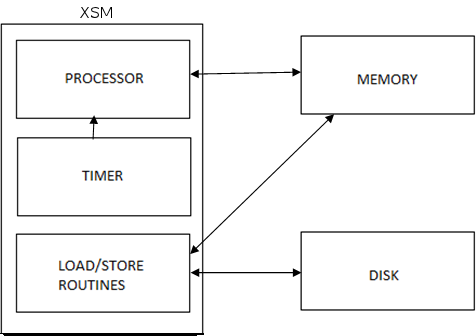
\includegraphics[scale=0.5]{block.png}
\end{center}
\caption{Components of the Machine}
\end{figure}


\begin{itemize}
\item Disk : It is a non-volatile storage that stores user programs (executables) and data files.
\item Memory : It is a volatile storage that stores the programs to be run on the machine as well as the operating system that manages the various programs.
\item Processor : It is the main computational unit that is used to execute the instructions.
\item Timer : It is a device that interrupts the processor after a pre-defined specific time interval.
\item Load/Store : It is a macro that performs the functionalities of DMA (Direct Memory Access) controller.
\end{itemize}






\section{Registers}

\subsection{Introduction}
The XSM architecture maintains 24 registers (strings).

\subsection{Register Set}
There are 16 General Purpose Registers (GPR), R0 - R15, of which R0 - R7 are Program Registers and R8 - R15 are Kernel Registers. There are 4 temporary registers T0 - T3 which are reserved for code translation. These registers cannot be used by the system programmer. In addition to these 20 registers there are 4 Special Purpose Registers(SPR) namely BP (Base Pointer), SP (Stack Pointer), PID (Process Identifier) and IP (Instruction Pointer).


\begin{center}
\begin{tabular}{|c|c|}
\hline Name & Register \\ 
\hline Program Register & R0-R7 \\ 
\hline Kernel Register & R8-R15 \\ 
\hline Temporary Registers & T0-T3 \\ 
\hline Base Pointer & BP \\ 
\hline Instruction Pointer & IP \\ 
\hline Stack Pointer & SP \\ 
\hline Process Identifier & PID \\
\hline
\end{tabular} 
\end{center}


\section{Memory}

\subsection{Introduction}

%\begin{figure}[hbtp]
%\begin{center}
%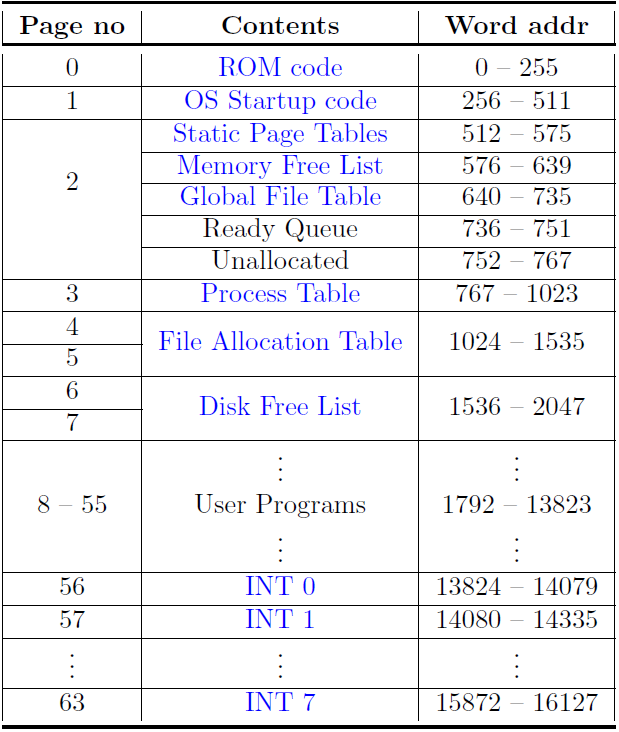
\includegraphics[scale=0.5]{memoryblockdiagram.png}
%\end{center}
%\caption{Main Memory Block Diagram}
%\end{figure}

\begin{itemize}
\item The basic unit of memory in XSM is a 16 character string.
\item The machine memory can be thought of as a linear sequence of strings.
\item A collection of 512 contiguous strings is known as a page.
\item The total size of the memory is 64 pages or 32768 (512 $\times$ 64) strings.
\item Each string in the memory is identified by the \textit{string address} in the range 0 to 32767 (512 $\times$ 64 - 1). Similarly, each page in the memory is identified by the \textit{page number} in the range 0 to 63.
\end{itemize}
\textbf{
\subsection{Address Translation}}

There are two kinds of memory addresses,\\

\begin{itemize}
\item Logical address : When a process runs, CPU generates address for the data accessed by this process. This address is called the Logical address.

\item Physical address : It is the actual location of the data in the main memory.
\end{itemize}

Address translation is the process of obtaining the physical address from the logical address. It is done by the machine in the following way. 
\begin{enumerate}
\item The logical address generated by the CPU is divided by the page size (512) to get the \textbf{logical page number}. The remainder is the \textbf{offset} of the data within that page.


\item A \textbf{page table} is used for address translation. It contains physical page numbers corresponding to each logical page number. The logical page number is used to index the page table to get the corresponding physical page number.

\item The \textbf{offset} is then used to refer to the word in the physical page containing the data.
\end{enumerate}






\section{Disk Storage}


\textbf{Block} : It is the basic unit of storage in the disk.\\

The disk can be thought of as consisting of a linear sequence of 512  blocks. The size of each block is equal to that of a page in the memory (512 strings). \\

Any particular block in the disk is addressed by the corresponding number in the sequence 0 to 511 known as the \textbf{block number}.


 \section{Instructions}

\subsection{Introduction}

Every instruction in XSM is 2 strings long. The instructions provided by the XSM architecture can be classified into privileged and unprivileged instructions. 

\subsection{Classification}

\subsubsection{Unprivileged Instructions}


\begin{enumerate}
\item MOV
\begin{itemize}
\item Immediate Addressing:\\
\textit{Syntax :} \texttt{MOV Ri, NUM/STRING}

Copies the \texttt{NUM/STRING} to the register \texttt{Ri}.

\item Register Addressing:\\
\textit{Syntax :} \texttt{MOV Ri, Rj}\\
Copies the contents of the register \texttt{Rj} to \texttt{Ri}.

\item Register Indirect Addressing:\\
\textit{Syntax }: \texttt{MOV Ri, [Rj]}\\
Copy contents of memory location pointed by \texttt{Rj} to register \texttt{Ri}.\\
\textit{Syntax :}\texttt{ MOV [Ri], Rj} \\
Copy contents of \texttt{Rj} to the location whose address is in \texttt{Ri}.
\item Direct Addressing:\\
\textit{Syntax :}\texttt{ MOV [LOC], Rj}\\
Copy contents of \texttt{Rj}  to the memory address \texttt{LOC}.\\
\textit{Syntax :} \texttt{MOV Rj, [LOC]}\\
Copy contents of the memory location \texttt{LOC} to the register \texttt{Rj}.
\end{itemize}


\item Arithmetic Instructions

\begin{itemize}
\item \texttt{ADD}, \texttt{SUB}, \texttt{MUL}, \texttt{DIV} and \texttt{MOD}.\\
\textit{General Syntax :} \texttt{OP Ri, Rj}\\
The result of \texttt{Ri} op \texttt{Rj} is stored in \texttt{Ri}. \texttt{Ri} and \texttt{Rj} should represent integers. Otherwise no operation is performed on the registers.

\item \texttt{INR\\}
\textit{Syntax :}\texttt{ INR Ri}\\
Increments the value of register \texttt{Ri} by 1.  \texttt{Ri} should represent an integer. Otherwise no operation is performed on \texttt{Ri}.

\item  \texttt{DCR}\\
\textit{Syntax :} \texttt{DCR Ri}\\
Decrements the value of register \texttt{Ri} by 1. \texttt{Ri} should represent an integer. Otherwise no operation is performed on \texttt{Ri}.

\end{itemize}


\item Logical Instructions
\begin{itemize}
\item \texttt{LT}\\
Syntax :\texttt{ LT Ri, Rj}\\
Stores 1 in \texttt{Ri} if the value stored in \texttt{Ri} is less than that in \texttt{Rj}. \texttt{Ri} is set to 0 otherwise. Strings can also be compared using \texttt{LT}

\item \texttt{GT}\\
Syntax : \texttt{GT Ri, Rj}\\
Stores 1 in \texttt{Ri} if the value stored in \texttt{Ri} is greater than that in \texttt{Rj}. \texttt{Ri} set to 0 otherwise. Strings can also be compared using \texttt{GT}

\item \texttt{EQ}\\
Syntax : \texttt{EQ Ri, Rj}\\
Stores 1 in \texttt{Ri} if the value stored in \texttt{Ri} is equal to that in \texttt{Rj}. Set to 0 otherwise. Strings can also be compared using \texttt{EQ}

\item \texttt{NE}\\
Syntax : \texttt{NE Ri, Rj}\\
Stores 1 in \texttt{Ri} if the value stored in \texttt{Ri} is not equal to that in \texttt{Rj}. Set to 0 otherwise. Strings can also be compared using \texttt{NE}

\item \texttt{GE} \\
Syntax : \texttt{GE Ri, Rj} \\
Stores 1 in \texttt{Ri} if the value stored in \texttt{Ri} is greater than or equal to that in \texttt{Rj}. Set to 0 otherwise. Strings can also be compared using \texttt{GE}

\item \texttt{LE}\\
Syntax : \texttt{LE Ri, Rj}\\
Stores 1 in \texttt{Ri} if the value stored in \texttt{Ri} is less than or equal to that in \texttt{Rj}. Set to 0 otherwise. Strings can also be compared using \texttt{LE} \\
\end{itemize}

\item Labels \\
Syntax : \texttt{LABEL \textit{labelname}} \\
Creates a label with a \texttt{\textit{labelname}}  which is a string. Labels are used in branching instruction to specify memory location of target instructions.


\item Branching Instructions\\
Branching is achieved by changing the value of the \texttt{IP} to the address of a specified \texttt{labelname}. 
 
\begin{itemize}
\item \texttt{JZ}\\
Syntax : \texttt{JZ Ri, labelname}\\
Jumps to \texttt{labelname} if the contents of \texttt{Ri} is zero.
\item \texttt{JNZ}\\
Syntax : \texttt{JNZ Ri, labelname}\\
Jumps to \texttt{labelname} if the contents of \texttt{Ri} is not zero.
\item \texttt{JMP}\\
Syntax : \texttt{JMP labelname}\\
Unconditional jump to address specified by \texttt{labelname}\\

\end{itemize}

\item Stack Instructions
\begin{itemize}
\item \texttt{PUSH}\\
Syntax : \texttt{PUSH Ri}\\
Increment \texttt{SP} by 1 and copy contents of \texttt{Ri} to the location pointed to by \texttt{SP}.
\item \texttt{POP}\\
Syntax : \texttt{POP Ri}\\
Copy contents of the location pointed to by \texttt{SP} into \texttt{Ri} and decrement \texttt{SP} by 1.\\
For both these instructions \texttt{Ri} may be any register except \texttt{IP}.
\end{itemize}

\item Subroutine Instructions\\
The \texttt{CALL} instruction copies the address of the next instruction to be fetched (\texttt{IP} + 2) on to location \texttt{SP} + 1, increments \texttt{SP} by one and transfers control to the \texttt{labelname} specified. The \texttt{RET} instruction restores the \texttt{IP} value stored at location pointed by \texttt{SP}, decrements \texttt{SP} by one and continues execution fetching the next instruction pointed to by \texttt{IP}. The subroutine instructions provide a neat mechanism for procedure evocations.
\begin{itemize}
\item \texttt{CALL}\\
Syntax : \texttt{CALL labelname}\\
Increment \texttt{SP} by 1, transfers \texttt{IP}+1 to location pointed to by \texttt{SP} and jumps to \texttt{LABEL}
\item \texttt{RET}\\
Syntax : \texttt{RET}\\
Sets \texttt{IP} to the value pointed to by \texttt{SP} and decrements \texttt{SP}.
\end{itemize}

\item Input/Output Instructions
\begin{itemize}
\item \texttt{IN}\\
Syntax : \texttt{IN Ri}\\
Transfers the contents of the standard input to \texttt{Ri}.
\item \texttt{OUT}\\
Syntax : \texttt{OUT Ri}\\
Transfers the contents of \texttt{Ri} to the standard output.\\
\end{itemize}

\item \texttt{START}\\
Syntax : \texttt{START}\\
\texttt{IP} will be initialised to this instruction automatically when a program is taken for execution.
\item \texttt{END}\\
Syntax : \texttt{END}\\
This instruction is marks the end of a program.

\item \texttt{INT}\\
Syntax : \texttt{INT n}\\
Generates an interrupt to the kernel with \texttt{n} (1 to 6) as a parameter. (Read Section \ref{sec:int})
\end{enumerate}


\subsubsection{Privileged Instructions}
There are four privileged instructions. They are:
\begin{enumerate}

\item \texttt{IRET}\\
Syntax : \texttt{IRET}\\

Set \texttt{IP} to the value pointed by \texttt{SP} and decrements \texttt{SP} by one. \texttt{IRET} does the same action as \texttt{RET}, but it tells the processor that the interrupt handler has finished. With the execution of the \texttt{IRET} instruction, interrupts are enabled. (Read Section \ref{sec:int})

\item \texttt{LOAD}\\
Syntax : \texttt{LOAD \textit{pagenum} \textit{blocknum}}\\
This instruction loads the block specified by the \texttt{\textit{blocknum}}, from the disk, to the page specified by the \texttt{\textit{pagenum}} in the memory. \texttt{\textit{blocknum}} and \texttt{\textit{pagenum}} should be numbers or registers containing numbers. Otherwise no action is performed.

\item \texttt{STORE}\\
Syntax : \texttt{STORE \textit{blocknum} \textit{pagenum} }\\ 
This instruction stores the page specified by the \texttt{\textit{pagenum}}, from the memory, to the block specified by the \texttt{\textit{blocknum}}in the disk. \texttt{\textit{blocknum}} and \texttt{\textit{pagenum}} should be numbers or registers containing numbers. Otherwise no action is performed.

\item \texttt{HALT}\\
Syntax : \texttt{HALT}\\
This instruction causes the simulator to halt immediately.
\end{enumerate}

\subsection{Processor Modes}
The XSM architecture is interrupt driven and uses a single processor. There are two privilege modes of execution, the user mode and the kernel mode. The privilege mode of execution is determined by the value of IP, i.e. the area in memory where the currently executing code executes. 


\begin{itemize}
\item User mode : Only unprivileged instructions can be executed in this mode. The value of IP cannot be changed in unprivileged mode.

\item Kernel mode : Both privileged and unprivileged instructions can be executed in this mode. 

\begin{center}
\begin{tabular}{|c|c|c|}
\hline Page Number & Privilege Space \\ 
\hline 0 & ROM Code \\ 
\hline 1 - 7 & Kernel Space \\ 
\hline 8 - 55 & User Space \\ 
\hline 56 - 63 &  Kernel Space (INT 0 - 7)  \\ 
\hline
\end{tabular} 
\end{center}

\end{itemize}

\section{Interrupts}
\label{sec:int}

\subsection{Introduction}
Interrupts are mechanisms by which the user code interrupts the execution of the processor and passes control to the kernel to accomplish low level functionalities like disk access, arithmetic exception handling etc.\\
\subsection{The \texttt{INT} instruction}
The instruction used to generate an interrupt is \texttt{INT}.\\
Syntax : \texttt{INT n}\\
The \texttt{INT} instruction passes control to the Interrupt Service Routine (ISR) for this interrupt located at the physical address computed using the value n.

Address computation is done as follows. The physical address of the ISR corresponding to interrupt number n is given by: 
\begin{verbatim}
Physical Address = (56 + n) x Page Size
\end{verbatim}
Note that the interrupts are disabled once this instruction is executed as interrupts cannot be executed in kernel mode.

\subsection{Types of Interrupts}
There are 8 interrupts (numbered from 0 to 7) supported by the XSM architecture. The interrupts 0 and 7 are hardware interrupts and the remaining interrupts (1 to 6) are software interrupts.\\

\textbf{Hardware Interrupts }

These interrupts cannot be called from user/kernel mode.
\begin{itemize}
\item \texttt{Interrupt 0} \\
It transfers control of execution, i.e. changes the value of IP to \textit{page number} 56 (address = 28672). This is the timer interrupt which interrupts the processor forcing a context switch. It contains the code for the scheduler of the operating system, which schedules the CPU time among the various active processes.

\item \texttt{Interrupt 7} : It transfers control of execution to \textit{page number} 63 (address = 32256). It is generated when the following exceptions occur:
\begin{enumerate}

\item Illegal memory access : occurs when any address generated by the process \textbf{does not} lie in the range \textbf{[0, 2047]}.
\item Arithmetic exception : occurs when divisor is 0.
\item Illegal instruction : occurs when an attempt is made to execute an instruction not belonging to the instruction set and also when the operands to the instruction is not legal. Eg: \texttt{MOV 4 R0}, \texttt{MOV IP 4} when executed in user mode. These instructions are considered illegal.
\item Stack overflow and stack underflow : Stack overflow occurs when the value in the \texttt{SP} register exceeds \textbf{2047} and stack underflow occurs when the value falls below \textbf{1536}.
\end{enumerate}
\textbf{Software Interrupts } \\
These interrupts are unprivileged and can be called from user mode.

\item \texttt{INT 1}  \\It transfers control of execution to \textit{page number} 57 (address = 29184)
\item \texttt{INT 2}  \\It transfers control of execution to \textit{page number} 58 (address = 29696)  
\item \texttt{INT 3}  \\It transfers control of execution to \textit{page number} 59 (address = 30208)
\item \texttt{INT 4}  \\It transfers control of execution to \textit{page number}  60 (address = 30720) 
\item \texttt{INT 5}  \\It transfers control of execution to \textit{page number} 61 (address = 31232)
\item \texttt{INT 6}  \\It transfers control of execution to \textit{page number} 62 (address = 31744).\

 
\end{itemize}


\end{document}